\justifying
\section{Water Crisis}
The growing global water crisis represents one of the greatest challenges that face humanity. This phenomenon, which affects different regions of the world to various degrees, has not only undermined the progress and the economic development of nations, but has also jeopardized basic human needs. The interaction between humans and water resources manifests itself in two dimensions: i) clean access to water and ii) safe access to sanitation services; (Fig.~\ref{fig1_intro}) the absence of either dimension can lead to a water crisis. In particular, the lack of access to clean water leads to economic losses such as lowered agricultural production, environmental effects (\textit{e.g.}, increased pollution of surface water and higher risks of fires), and social costs that negatively affect public health. On the other hand, the lack of sanitation services increases exposure to waterborne diseases such as diarrheal infections and compromises the quality of the watershed. To understand the extent of the magnitude of the water crisis across the world, it is beneficial to provide the following two numbers: 2.1 billion and 4.5 billion. These numbers refer to the number of people across the world who do not have access to safe drinking water and sanitation services, respectively.\cite{WB}
\begin{figure}
  \centering
  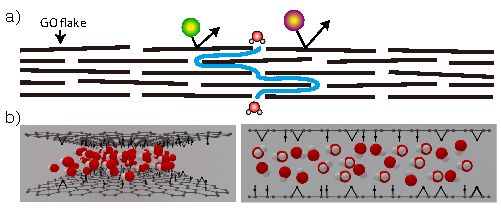
\includegraphics[width=6in]{intro/Fig1.pdf}
  \caption{\textbf{Water-humans interaction}. Access to clean water and safe sanitation services are the pillars of sustainable development. Climate change and change in water demand are deeply influencing the water-humans interaction.}
  \label{fig1_intro}
\end{figure}
 
Currently, two anthropogenic phenomena further stress the relationship between humans and water and thereby worsen the water crisis. First, climate change exacerbates the risks associated with variations in the distribution and availability of water resources. It is responsible for the severity and frequency of extreme events. For example, the increased variability in precipitation patterns leads to changes in the hydrological cycle, which affects the rate at which the aquifers recharge and the availability of fresh water. As a consequence, in recent years, we have witnessed severe droughts in California, Brazil, China, Iran, South Africa, just to mention some. \cite{van2016drought} Second, we are observing a change in the demand for water. Water usage is six times greater than it was a century ago, and by 2050, the global water requirement is projected to increase by 55\%, mainly due to growing demands from manufacturing, thermal electricity generation and domestic use \cite{UN2015}. Since the increase in water use is also influenced by increases in population and income, which are projected to flatten only by the end of this century \cite{Gerland234}, global water withdrawal will increase by a staggering 150\% by 2095. \cite{DAVIES2013296}
Groundwater plays a pivotal role in the global water supply. The world's most extracted material, groundwater is withdrawn at a rate of $\approx1000$ km\textsuperscript{3}/year. It accounts for approximately 26\% of total global water withdrawal \cite{Unesco} and more than 2 billion people rely exclusively on groundwater to satisfy their basic needs.\cite{doi:10.1002/9781118971772.ch7} Agriculture also relies heavily on groundwater and accounts for 43\% of the total withdrawal. High rates of withdrawal lead to unsustainable use of groundwater with an estimated 20\% of the aquifers being over-exploited, leading to water-stressed regions.\cite{UN2015} Today, 4.3 billion people live in water-stressed areas for at least 1 month out of the year. (Note that an area is defined to be water-stressed when the amount of available freshwater per person per year is between 1000 and 1700 m\textsuperscript{3}. \cite{mekonnen2016four})\\
Needless to say, it is paramount to look at innovative technologies that can safely supply water without undermining hydrological cycles and ecosystems, thus reducing the stress on freshwater bodies. In this sense, wastewater reclamation can be a valid alternative to the withdrawal of groundwater or even worse fossil water.
 
\section{Wastewater Reclamation}
Wastewater (WW) treatment decreases environmental impact and protects humans from risks associated with municipal and industrial water discharge. WW treatment plants are designed to remove contaminants from water via three treatments (Fig.~\ref{fig2_intro}). i) Primary treatments consist of physical methods that either rely on gravitational force to sediment heavy solids and particulates or scrape away grease and lighter solids that float. ii) Secondary treatments remove dissolved and suspended organic matter via biological treatment, in which bacteria and protozoa consume biodegradable, soluble organic contaminants. iii) Tertiary treatments mainly focus on the removal of nitrogen and phosphorus via biological oxidation or chemical precipitation. Finally, before discharging the treated WW to the receiving body of water (sea, river, lake, etc.), a disinfection process via chlorination, ultraviolet irradiation, or ozonation reduces the number of microorganisms in the water to below an acceptable threshold. \cite{qasim2017wastewater}
\begin{figure}
  \centering
  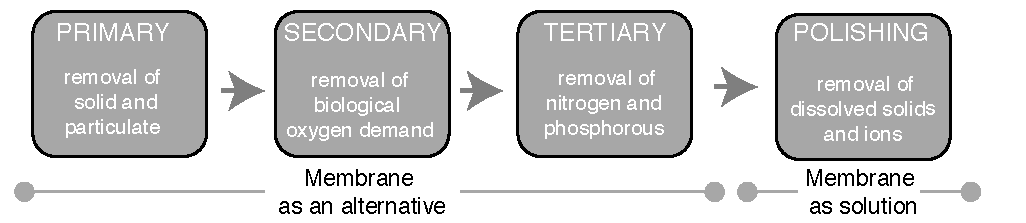
\includegraphics[width=6in]{intro/Fig2.pdf}
  \caption{\textbf{Wastewater treatment.} In the primary, secondary, and tertiary treatments membranes can be used as a valid alternative to currently used technologies. Membranes are the only solution for the polishing stage required for wastewater reclamation.}
  \label{fig2_intro}
\end{figure}
 

WW can be further treated during a polishing stage that removes dissolved solids and ions, thus reclaiming the water for agriculture, industrial, or drinking purposes. This stage is usually recommended because it recovers water within the anthropogenic cycle and avoids the use of new freshwater from the natural cycle. In this sense, WW reclamation is an example of a circular economy, that short-circuits the transport of water through the natural water cycle  thus decreasing our environmental impact. Furthermore, reclaimed WW is characterized by a relatively constant production during the year, due to its source being dependent not on natural hydrological cycles, but on the production of municipal sewage. \cite{pintilie2016urban}\\
From an energy perspective, WW reclamation tends to be advantageous compared to other technologies such as desalination or groundwater extraction. WW reclamation uses a total of $2-3$ kWh/m\textsuperscript{3},\cite{guerrini2017energy} of which 1 kWh/m\textsuperscript{3}\cite{qasim2017wastewater} is the energy used by primary and secondary treatments, which are mandated by legislation.\cite{hunter2016enforcing} As a result, as low as 1 kWh/m\textsuperscript{3} is needed for the polishing stage to reclaim water, which is significantly lower than the energy used by desalination plants ($4-5$ kWh/m\textsuperscript{3}) \cite{elimelech2011future,stillwell2016predicting} or the extraction and transportation of groundwater to water-stressed areas (\textit{i.e.}., up to 4 kWh/m\textsuperscript{3} for Southern California).\cite{schneir2010} Although WW reclamation seems to be the ideal solution in terms of energy cost and environmental impact, there are a few obstacles to its implementation, including insufficient public acceptance and lack of an uniform legislation. In terms of technical performance, the main challenges are related to the functionality of the membranes used during the polishing stage.



\section{Membranes}
Membrane filtration is a physical process in which a semipermeable material separates substances when a driving force is applied. In the case of water treatment applications, the feed is made up of water and dissolved contaminants (\textit{e.g.}, salts). When the water is filtered through the membrane and the contaminants are rejected, the permeate is collected on the other side of the membrane. Membrane filters can be operated in dead-end configurations, but more common are cross-flow configurations where the concentrate water can be recirculated at high velocity across the face of the membrane (see Fig.~\ref{fig3_intro}).\cite{baker2004overview}
\begin{figure}
  \centering
  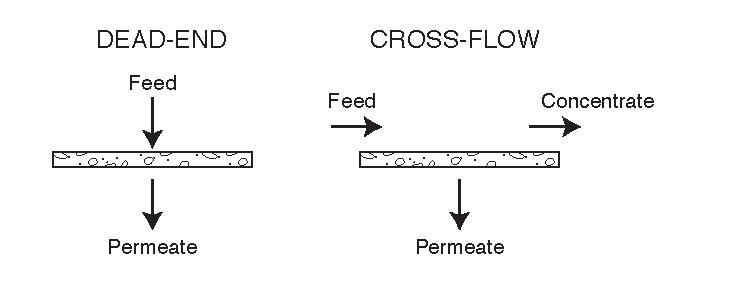
\includegraphics[width=4.5in]{intro/Fig3.pdf}
  \caption{\textbf{Membranes operation.} Dead-end filtration requires the flow of water to be perpendicular to the membrane surface. In cross-flow operations, the feed flow travels tangentially across the surface of the membrane.}
  \label{fig3_intro}
\end{figure}
 
Several forces can be used to drive the feed across the membrane: pressure, concentration, and temperature, just to mention some. In water technology, pressure-driven membrane filtration is an increasingly-used process and membranes are classified into four categories based on pore size. i) Microfiltration (MF) membranes are used to remove large suspended solids ranging from 0.1 to 10 $\mu$m and larger micro-organisms like protozoa and bacteria. ii) Ultrafiltration (UF) membranes are used to remove viruses and organic solids ranging from 10 to 100 nm. iii) Nanofiltration (NF) membranes are used to remove smaller dissolved solids and multivalent ions and have a pore size between 1 and 20 nm. iv) Reverse osmosis (RO) membranes remove ions and are characterized by sub-nanometer pore sizes. Table~\ref{tbl1_intro} summarizes the characteristics of each type of membrane.

\begin{table}[ht]
 \begin{center}
 \caption{\textbf{Membranes characteristics.}}
  \label{tbl1_intro}
  \begin{tabular}{ccccc}
        \hline
        Membrane & Pore size & Removal & Pressure & Material\\ 
         & (nm) & Application & (bar) & Material\\
        \hline
        MF & $10-10000$ & Bacteria, & $0.5-1$ & polyvinylidene difluoride,\\
         & &  protozoa, algae &  &  polyethersulfone\\
         UF & $10-100$ &Large particles,  & $0.7-10$ & polyvinylidene difluoride,\\
         & &  viruses, proteins &  &  polysulfone, polyacrylonitrile\\
         & &  &  &  polypropylene\\
        NF & $1-20$ &Dissolved organics,   & $5-30$ & Thin film composite\\
         & &  multivalent ions&  & (polyamide as selective layer)\\
         RO & $<1$, & Monovalent ions   & $30-50$ & Thin film composite\\
         & &  &  & (polyamide as selective layer)\\
        \hline
  \end{tabular}
 \end{center}
\end{table}




Membrane technology is a valid alternative to traditional processes in drinking and WW treatment plants. A clear example is given by the membrane bioreactor, which can be used instead of primary and secondary treatments in domestic WW plants. On the other hand, for water reclamation, membranes are the only viable solutions and the typology of membranes used depends on the WW feed quality and on the reclamation purposes (urban, agricultural, environmental, potable uses, etc.). High water quality requirements (\textit{e.g.}, direct potable reuse) typically consist of conventional wastewater treatment followed by UF, NF, and/or RO and, finally, disinfection by UV light or ozone.\\
NF and RO technology is dominated by polyamide polymeric membranes, which are susceptible to membrane fouling, the Achilles' heel of membrane separations.\cite{safarpour2015thin} Fouling is defined as the accumulation of particles on the membrane and, in case of biological fouling, we observe a series of events including cell attachment, cell growth, and the production of extracellular polymeric substances. Fouling can be divided into reversible and irreversible fouling based on the attachment strength of particles to the membrane surface. Reversible fouling can be mitigated by shear force, backwashing, and the introduction of periodic cleaning steps into the filter's operational cycle. However, in terms of biological fouling, sodium hypochlorite solution is used as a cleaning agent, which can cause membrane damage.\cite{chae2015graphene} For this reason, scientific research is currently trying to address the problem by investigating how to incorporate materials resistant to chemicals such as cleaning agents into the membrane. In the last five years, one of the materials that have received a lot of attention from the research community is graphene oxide (GO).

\section{Graphene Oxide}
GO is a single layer of carbon atoms arranged in a hexagonal (sp\textsuperscript{2}) lattice decorated with oxy-functionalities (Fig.~\ref{fig4_intro}) which make this material a mixed blessing.\cite{Dreyer2010} On the one hand, researchers can modify the amount of oxy-functionalities through oxidation and reduction processes,\cite{Pei2012} thus tuning the GO chemistry for a particular application. On the other hand, the oxy-functionalities can react with the surrounding environment to make the GO a metastable material without defined stoichiometry.\cite{hou2015photochemical} This phenomenon can make it difficult to reproduce and compare results within the research community, which is a critical step in the translation of GO applications from ''lab-scale'' to ''industrial-scale''.

\begin{figure}
  \centering
  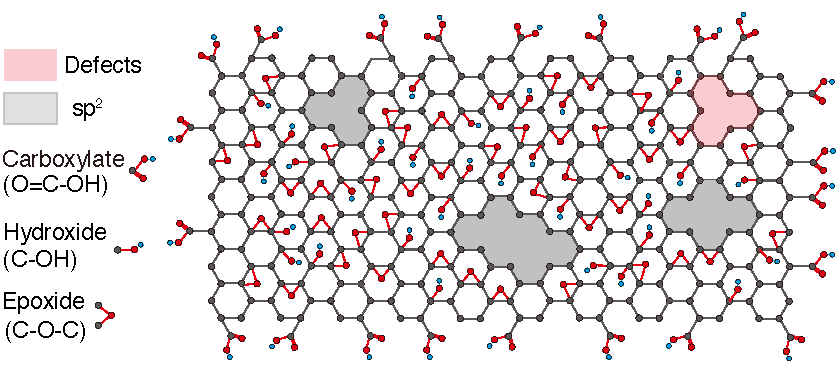
\includegraphics[width=6in]{intro/Fig4.pdf}
  \caption{\textbf{Graphene oxide structure.} Atom-thin carbon structure decorated with oxy-functionalities.}
  \label{fig4_intro}
\end{figure}

GO displays unique properties (see Fig.~\ref{fig5_intro})  such as near-atomic thickness, functionalization possibilities due to the presence of reactive oxygen species,\cite{chen2012graphene} scalable synthesis processes,\cite{akbari2016large}  and the possibility of controlled deposition of nanofilms through several techniques. This has led researchers to propose the use of GO in fields such as separation process,\cite{mi2014graphene} electronics,\cite{eda2008large} energy storage,\cite{le2011graphene} sensors,\cite{drewniak2016studies} just to mention a few; the reader can refer to literature reviews to gain a more complete view of GO applications\cite{georgakilas2016noncovalent,sun2016recent,fathizadeh2017graphene}

\begin{figure}
  \centering
  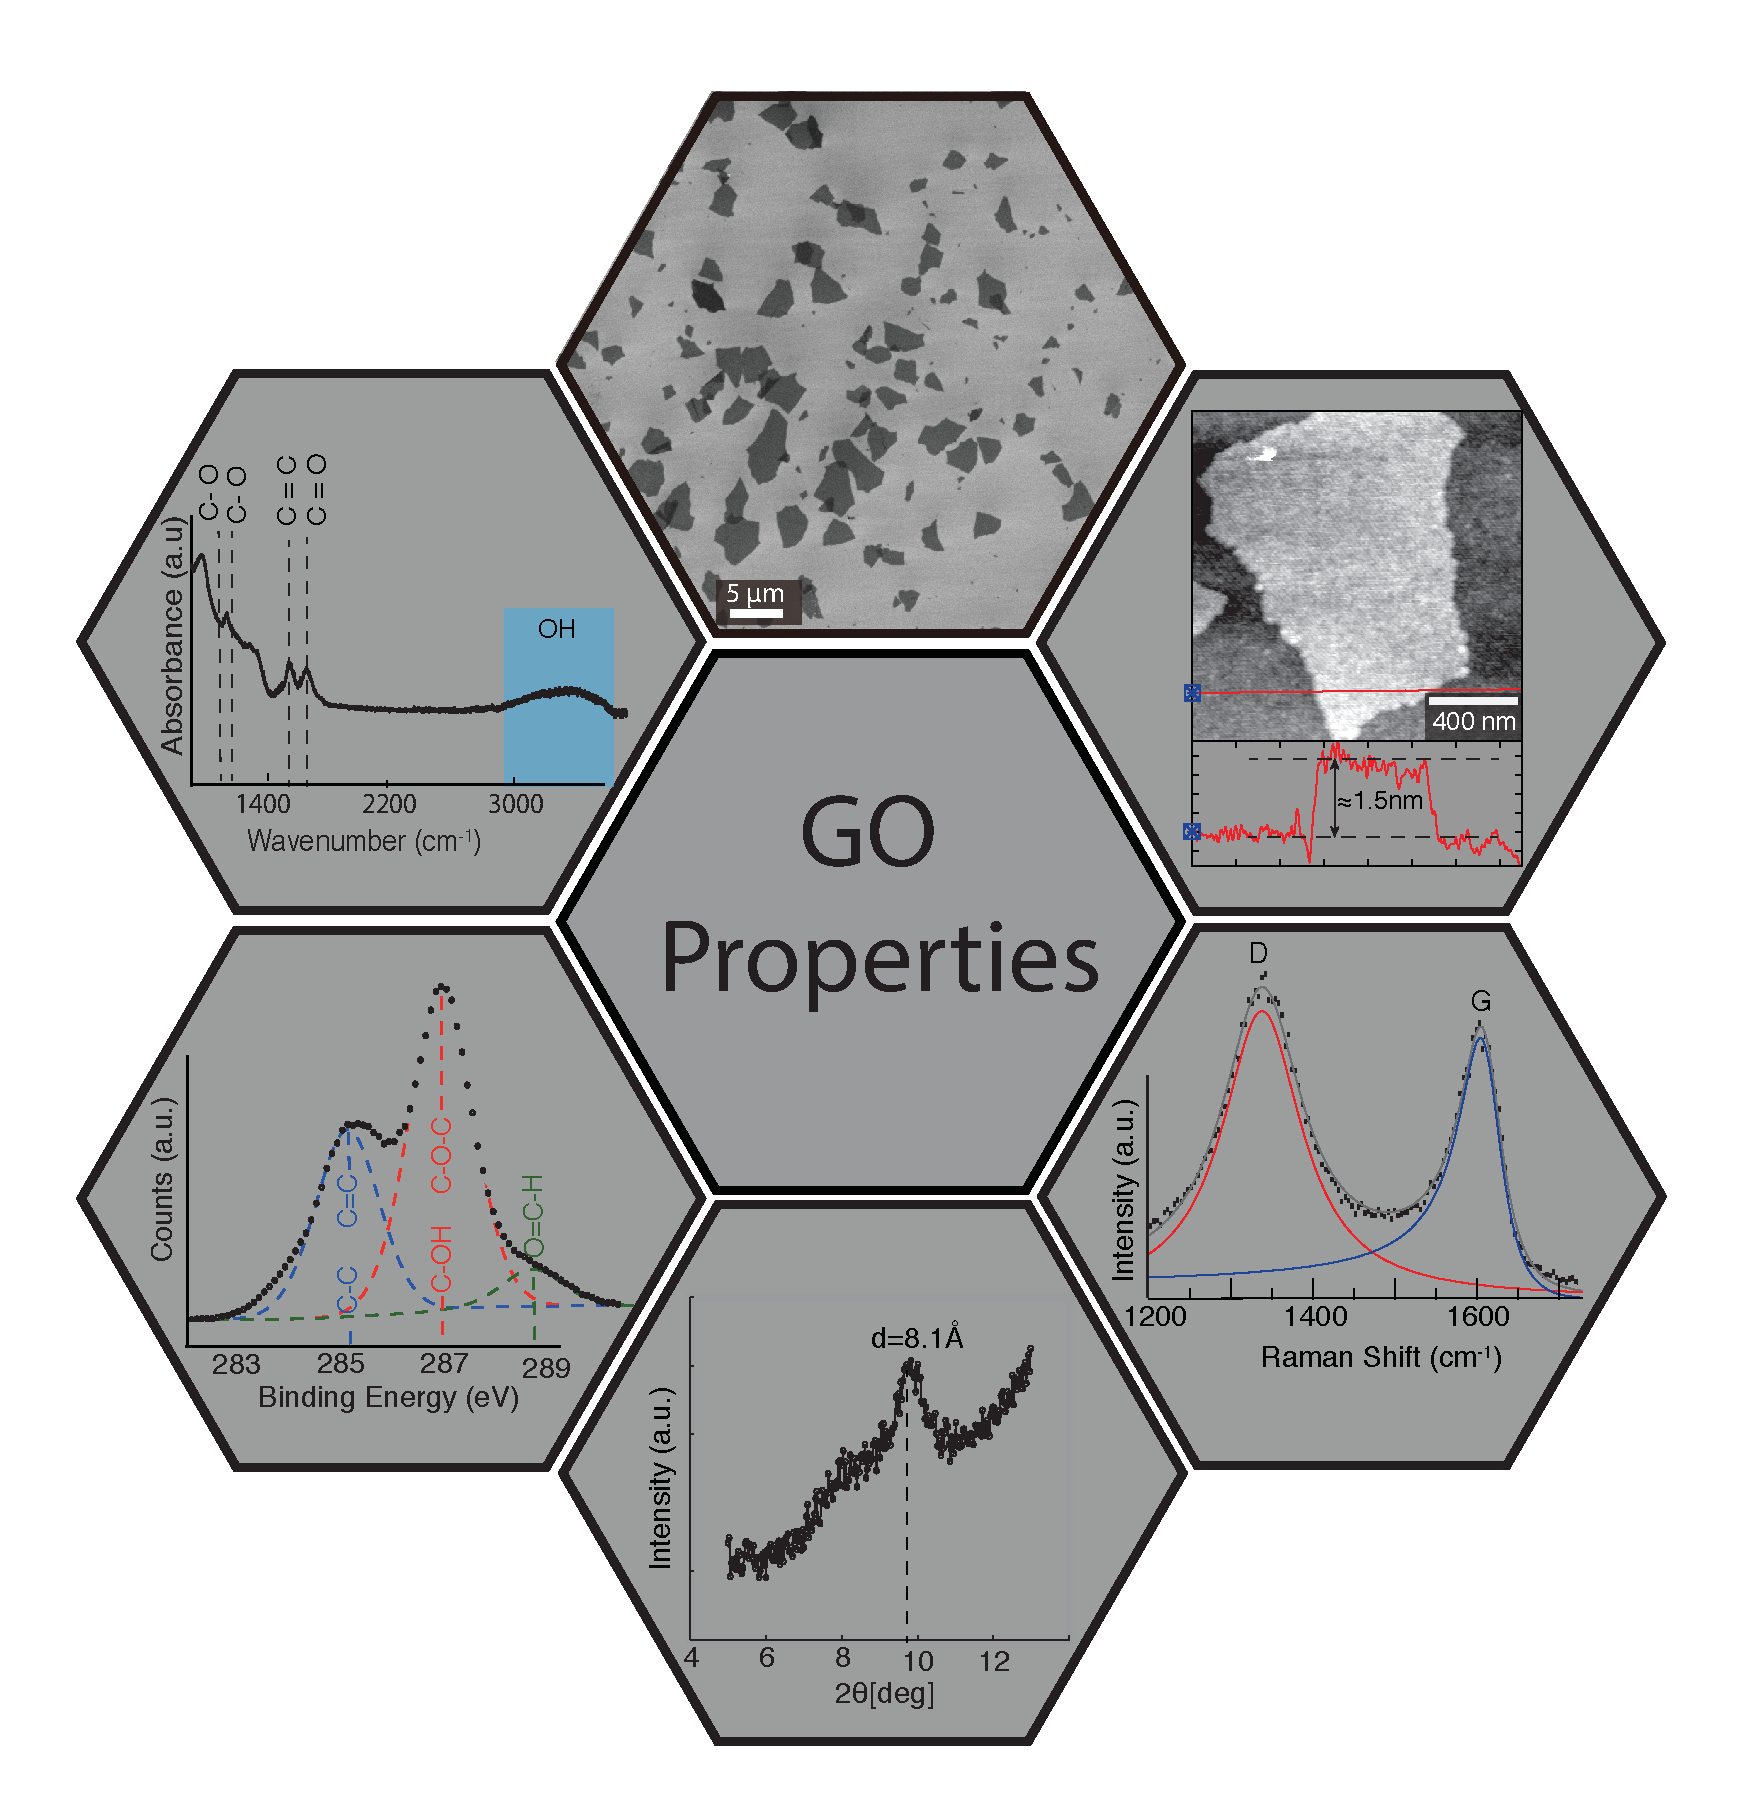
\includegraphics[width=5.5in]{intro/Fig5.pdf}
  \caption{\textbf{Graphene oxide properties.} Clockwise from top: scanning electron microscope image displays the micrometer-sized GO flakes, atomic force microscope scan highlights the GO monolayer nature, Raman spectrum confirms the sp\textsuperscript{2} bonding, X-ray diffraction spectra reports the separation distance between GO flakes, X-ray photoelectron spectra quantifies the presence of oxy-functionalities, Fourier transform infrared spectrum corroborates the presence of oxy-functionality.}
  \label{fig5_intro}
\end{figure}

 
Regarding separation processes, the use of two-dimensional graphitic materials was first proposed by Tanugi and Grossman using classical molecular dynamics simulations in 2012.\cite{cohen2012water} In their investigation, they showed that  single layer graphene could effectively filter ions from water. Researchers at MIT then experimentally engineered Tanugi and Grossman's proposed design by creating pores in graphene fabricated via chemical vapor deposition (CVD).\cite{o2012selective} Concurrently, Nobel prize winner Geim was investigating the possibility of using stacked GO flakes instead of monolayer graphene.\cite{nair2012unimpeded} Although the results of the article remain controversial, the paper sparked an incredible amount of interest in the use of GO for water treatment applications. The surge was mainly driven by the ease of fabricating GO. In particular, GO can be synthesized at scale and in a cost-effective manner, which is hard to obtain in the synthesis of pristine graphene via bottom-up approaches (\textit{e.g.}, CVD).\cite{eletskii2011graphene}\\
Any major breakthrough in science brings with it new avenues of inquiry. This thesis addresses some of the key questions raised by recent developments in the field of GO for water treatment applications. 

\section{Thesis Overview}
The work presented in this dissertation focuses on the nanoengineering of GO for water treatment applications with emphasis on its chemo-morphological properties and their effects on implementation.\\
Chapter 2 analyzes the state of the art for GO membranes and elucidates challenges in the implementation of GO in large-scale water treatment applications. The challenges presented in this chapter will be tackled in the following chapters to offer an in-depth look at the GO landscape.\\
Chapter 3 contains a discussion of GO's chemo-morphological properties, offering high-throughput characterization methods. In this chapter, I also suggest a GO standardization method to enable the leap of this nanomaterial from lab to industry.\\
Chapters $4-6$ offer GO applications for water treatment applications. In particular, Chapter 4 focuses on the fabrication of GO nanoscrolls and the tuning of their dimensions via ultrasound irradiation. Chapter 5 is centered around the creation of GO membranes whose chemo-morphological properties can be finely controlled. The properties act as knobs that dictate the transport of water in GO nanochannels. Computational fluid dynamics simulations based on mesoscale approaches provide supporting analysis. Chapter 6 reports the first fully carbon membrane in which the elemental composition of all materials is > 75\% carbon and the repeating units (\textit{i.e.},. monomers) of the polymer have been replaced with elemental carbon architectures. In future directions, we tried to assess GO toxicity in order to limit risks connected to human exposure. 

